\section{Changing the numerical rank}
The worst materials prefix contains 72 distinct feature vectors in 73 rows. Its largest singular value is 47.94, its smallest retained value is $7.71\times10^{-12}$, and its default cutoff is $8.62\times10^{-13}$. The last retained direction carries more than 99.9999\% of the squared coefficient norm. These observations motivated two post-hoc checks. Both use the original data, splits and seeds. Neither benchmark was used to select a cutoff for deployment.

\subsection{Recomputing predictions on the same rows}
For each of the 1,500 materials prefixes, we keep the original preprocessing and solver and retain the singular values exceeding
\[
    \tau_c=\max(\tau_0,c s_1),\quad c\in\{0,10^{-12},10^{-10},10^{-8},10^{-6}\}.
\]
For every cutoff we restore the intercept and score the resulting predictions on all 4,392 held-out rows. This changes the estimator for affected prefixes and keeps all 100 repetitions in each curve. The default calculation reproduces all 1,500 archived minimum-norm losses exactly on the study system. Table~\ref{tab:cutoff} reports all five specifications, including settings for which the peak moves back toward smaller $n$.

\begin{table}[htb]
\centering
\caption{Materials sensitivity across the full grid. The changed count is relative to the default among 1,500 fits. Peak locations maximize the indicated sample summary over the 15 observed sizes. The last column measures concentration at the mean peak.}
\label{tab:cutoff}
\begin{tabular}{lrrrrr}
\toprule
Relative floor $c$ & Changed & Mean peak $n$ & Peak mean MSE & Median peak $n$ & Largest share\\
\midrule
\tableinput cutoff_rows.tex
\bottomrule
\end{tabular}
\end{table}

At $c=10^{-12}$ only repetition 5 changes at $n=73$. Its MSE falls from $3.24\times10^{21}$ to $2.64\times10^{15}$. The other 99 losses at that size are identical. The mean drops from $3.24\times10^{19}$ to $2.69\times10^{16}$ and the median stays at $1.40\times10^6$. Across the full grid the highest mean moves to $n=83$, on the other side of $p+1=82$. By comparison, at $c=10^{-8}$ the two highest means at $n=73$ and 81 differ by less than 0.1\%. Figure~\ref{fig:cut} shows both the size of the vertical change and the fragility of the horizontal ordering. Even after imposing the largest floor, the peak mean MSE is above $4\times10^7$.

Deleting one entire training trajectory at a time keeps the pairing across sizes. At the default cutoff, 99 deletions leave the mean peak at 73 and one moves it to 83. At $c=10^{-10}$ all 100 deletions leave the peak at 81. On comparing the two sizes singled out by the first change of cutoff, the default paired mean difference $L_{73}-L_{83}$ is $3.21\times10^{19}$, with a descriptive pointwise interval of $[-3.19,9.61]\times10^{19}$. At $c=10^{-12}$ it is $-1.55\times10^{17}$, with interval $[-4.49,1.40]\times10^{17}$. The sign reversal describes the finite archive. Neither interval resolves an ordering of the two permutation expectations, and the sizes were chosen after inspecting the curves.

\begin{figure}[htb]
\centering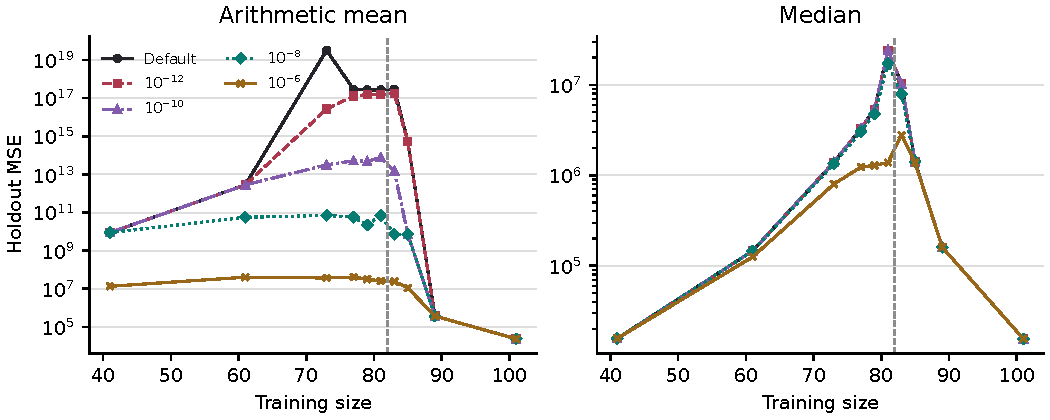
\includegraphics[width=.96\linewidth]{../replication/summary/cutoffs.pdf}
\caption{Recomputed minimum-norm losses on the materials holdout. The near-boundary part of the grid is expanded horizontally. Overlapping lines indicate identical or similar loss summaries. The vertical line marks $p+1=82$.}
\label{fig:cut}
\end{figure}

\subsection{Was the training matrix exactly singular?}
A floating-point SVD alone cannot establish the exact rank of a matrix of recorded decimal numbers. Let $A$ contain the original decimal features of a prefix, interpreted as rationals. Define $B$ by subtracting its first row from every other row. The rows of $B$ span the row space of the centered $A$: every centered row is a linear combination of differences, and subtracting two centered rows recovers their difference. Column scaling by nonzero factors preserves rank. With $m$ distinct decimal rows, $u=\min(p,m-1)$ is therefore an upper bound on the centered rank.

For a lower bound we reduce each rational entry modulo the prime $q=1{,}000{,}000{,}007$ and perform Gaussian elimination on the row differences over $\mathbb F_q$. Finite decimal denominators have only prime factors 2 and 5, so reduction is defined. A nonzero minor modulo $q$ implies a nonzero rational minor. The field rank $\ell$ is consequently a deterministic lower bound, and $\ell=u$ certifies the rank exactly. An inconclusive bound would require further work. This check uses only the printed features.

We applied it to every prefix with a default-retained singular value below $10^{-10}s_1$. There were 25 such fits across eight distinct permutations. All 25 bounds met. In 21 fits the default numerical rank equaled the certified rank. In four it was one smaller. For the worst prefix both bounds are 71 and the default fit retained 71 directions. Raising the floor to $10^{-12}s_1$ leaves rank 70. The published decimals therefore support 71 independent centered directions even though retaining the last one is disastrous for prediction. This rank result gives neither the exact magnitude of the smallest singular value nor the precision of the underlying materials measurements.
